\documentclass[12pt]{article}
\usepackage[margin=1in]{geometry}
\usepackage{mdframed}
\usepackage{subcaption}
\usepackage{amssymb}
\usepackage{amsmath}
\usepackage{mathtools}
\usepackage[ruled,vlined,linesnumbered]{algorithm2e}
\definecolor{lapislazuli}{rgb}{0.15, 0.38, 0.61}
\newcommand{\CommentFont}[1]{\texttt{\color{lapislazuli}#1}}
\SetCommentSty{CommentFont}
\SetKwComment{Comment}{// }{}
% Custom colors
\usepackage{color}
\definecolor{deepblue}{rgb}{0,0,0.5}
\definecolor{deepred}{rgb}{0.6,0,0}
\definecolor{deepgreen}{rgb}{0,0.5,0}
% Default fixed font does not support bold face
\DeclareFixedFont{\ttb}{T1}{txtt}{bx}{n}{12} % for bold
\DeclareFixedFont{\ttm}{T1}{txtt}{m}{n}{12}  % for normal
\usepackage{listings}
\usepackage{url}

\usepackage{booktabs}
\usepackage{hyperref}

\usepackage{tikz}
\usetikzlibrary{shapes,arrows,automata,positioning,cd}
\tikzset{
  cfgedge/.style   = {black, ->, >=stealth},
  forward/.style = { blue, ->, >=angle 45},
  backward/.style = { red, densely dashed, ->, >=latex' },
  backwardleft/.style = { red, densely dashed, <-, >=latex' },
}
\usepackage{xcolor}

\newcommand{\cfgarrow}{\mathbin{\tikz[baseline]\draw[cfgedge,yshift=0.6ex] (0,0) -- (.9em,0);}}
\newcommand{\forwardarrow}{\mathbin{\tikz[baseline]\draw[forward,yshift=0.6ex] (0,0) -- (1em,0);}}
\newcommand{\backwardarrow}{\mathbin{\tikz[baseline]\draw[backward,yshift=0.6ex] (0,0) -- (.95em,0);}}
\newcommand{\dom}{\underline{\gg}}


\begin{document}
\lstset{
language=C,
basicstyle=\ttfamily\small,
keywordstyle=\ttb\color{deepblue}\small,
emph={foo,bar,assert,baz},          % Custom highlighting
emphstyle=\ttb\color{deepred}\small,    % Custom highlighting style
stringstyle=\color{deepgreen}\small,
frame=tb,                         % Any extra options here
showstringspaces=false            % 
}

\begin{center}
    \bigskip
    {\LARGE ECS 240 Programming Languages} \medskip
    
    {\Large Homework 1} \bigskip

\end{center}

\section*{About This Assignment}

\begin{itemize}
  \item This assignment tests you on your understanding of dominators and
  control dependence.
  \item To complete the assignment (i)~modify \texttt{hw1.tex}, (ii)~create
  the corresponding PDF document (using pdflatex, for example), and
  (iii)~submit the pdf electronically via Gradescope by the due date; see
  \href{https://www.gradescope.com/get_started#student-submission}{this page}
  and
  \href{http://gradescope-static-assets.s3-us-west-2.amazonaws.com/help/submitting_hw_guide.pdf}{this
  document}. Your assignment will not be graded and you will receive no
  points if you do not follow these instructions. 

  \item \textbf{When submitting the assignment on Gradescope, please mark
  which page corresponds to each question on the assignment.}  Your
  assignment will not be graded and you will receive no points if you do not
  mark the pages.      

  \item The  \LaTeX\ source has \texttt{TODO}~comments to clearly indicate
  where changes need to be made. 
  \item The \verb=\vspace= commands can be safely commented out.
  \item This assignment can be worked on in a group of at most three. Enter
  the names and email addresses of the team members in the space provided
  below.
\end{itemize}

\begin{mdframed}
  Team members:
  \begin{itemize}
    %TODO
    \item Soham Kolhatkar, sakolhatkar@ucdavis.edu % Enter name and email address of first team member.
    \item Divyansh Rajesh Jain, drajeshjain@ucdavis.edu % Comment out this line if working individually.
    %\item Name, email address % Comment out this line if working in pairs.
  \end{itemize}
\end{mdframed}

\newpage
\begin{enumerate}

  
  \item Prove the following about the dominator relation $\dom$:
  \begin{enumerate}
    \item (5 points) If $a \dom b$ and $b \dom c$, then $a \dom c$
    (transitivity).
    \begin{mdframed}
      %\vspace{2em}
      We can prove this directly. We assume that the definition of the dominator relation holds true.

      The definition of $a \dom b$ (a dominates b) means every path from the start node to node $b$ passes through node $a$."

    Similarly, by the same definition, Every path from the start node to node $c$ passes through node $b$."
    

    We can use the definitions to say the following.

    Let $p$ be any path from the start node to $c$. If $a \dom b$, then $p$ must go through $a$ to get to $b$. Additionally if $b \dom c$,  then $p$ must go through $b$ to get to $c$. Therefore, since both are true, then  then $p$ must go through $a$ to get to $c$

    

    Since all paths must go through node $a$ to get to $b$ and all paths must also go through $b$ to get to $c$, by definition of the dominator relation all paths from start  must go through $a$ to get to $c$. 

    Through this we can see, by the defintion of the dominator, we can say that if $a \dom b$ and $b \dom c$, then $a \dom c$.
      
    \end{mdframed}

    \item (5 points) It is never possible that both $a \dom b$ and $b \dom
    a$, if $a \neq b$ (anti-symmetry).
    \begin{mdframed}
      %\vspace{2em}

       We can prove this below through contradiction.
        \vspace{0.5em}
        
       Assume for contradiction that it is possible that $a \dom b $ and $ b \dom a$ and $ a \neq b$. By definition of the dominator relation, this means all paths $p$ from entry to $b$ must pass through $a$. In other words, all paths must \textbf{first} go through $a$ before reaching $b$.
       \vspace{0.5em}

       Similarly, all paths $p$ from entry to $a$ must pass through $b$. In other words, all paths must \textbf{first} go through $b$ before reaching $a$.

\vspace{0.5em}
    Consider a path $p$ from entry to $b$ where all such $p$ pass through $a$, and  $a \ne b$, and  $a \dom b$. By definition of a dominator, $a$ must appear \textbf{before} $b$ for $a \dom b$ since $a \ne b$ and since $p$ is a sequence of nodes.
\vspace{0.5em}

    Vice versa, consider a path $p$ from entry to $a$ where all such $p$ pass through $b$ , and  $a \ne b$ and $b \dom a$. By definition of a dominator, $b$ must appear \textbf{before} $a$ for $b$ to dominate $a$ since $a \ne b$ and since $p$ is a sequence of nodes.
    
\vspace{0.5em}

       However both of these statements cannot be true at once since in the sequence of nodes in $p$ one has to come before the other.

       Thus, it is impossible for the above property to hold unless $a = b$.
      
    \end{mdframed}

    \item (5 points) If $a$ and $b$ are two dominators of $n$, then either
    $a \dom b$ or $b \dom a$ must hold.
    \begin{mdframed}
      %\vspace{2em}
      We can prove this below through contradiction.
      \vspace{0.5em}
      
      
      Assume for contradiction that $a$ and $b$ are two dominators of $n$, then \textbf{neither}
    $a \dom b$ nor $b \dom a$ will hold.
    \vspace{0.5em}

    By the definition of the dominator relation, we know that $a \dom n$ means that for all paths $p$ from entry to $n$, $p$ must pass through $a$.
    \vspace{0.5em}

    Similarly, we know that $b \dom n$ means that for all paths $p$ from entry to $n$, $p$ must pass through $b$.

    \vspace{0.5em}

    Given any path $p$ from entry to $n$, we know from the definitions above that $p$ must pass through both $a$ and $b$, and a path consists of a sequence of nodes, so that means either $a$ must come before $b$ or $b$ must come before $a$.
\vspace{0.5em}


    Suppose $a$ comes before $b$ on all paths $p$. If $a$ always comes before $b$ on every path to $n$, and all such paths go to $b$, then $a \dom b$ — because all paths to b go through a. The same applies if $b$ were to appear before $a$ in $p$.
    
    \vspace{0.5em}

    This however contradicts our original assumption where \textbf{neither} $a \dom b$ nor $b \dom a$ will hold. Thus we have completed our proof
    
    \end{mdframed}

    \item (5 points) Each node $n$ except the entry has a unique
    \emph{immediate dominator} --- the dominator that appears closest to $n$
    along any acyclic path from the entry to $n$.
    \begin{mdframed}
      %\vspace{2em}

      We can prove this through a contradiction proof.

      \vspace{0.5em}

      Assume for contradiction that each node $n$ except the entry \textbf{does not} have a unique immediate dominator.

      \vspace{0.5em}
            Let there be two distinct dominators of $n$, $a$ and $b$ and that we have any path $p$ from the entry node to $n$. We know from the previous proof that if there are two nodes $a$ and $b$ such that $a \dom n$ and $b \dom n$, then either
            $a \dom b$ or $b \dom a$ must hold. Since we know this to be true, we can say that either $a$ comes before $b$ in $p$ or vice versa.
                   
      \vspace{0.5em}
            Suppose $a$ appears before $b$ in $p$. This means that all paths from entry to $n$ must pass through $a$ and all paths from $a$ to $n$ must pass through $b$. However, if $a$ appears before $b$ and both dominate $n$, then this means that one of the nodes is not the \textbf{immediate} dominator of $n$ because one dominator is closer to $n$ in $p$. This contradicts our assumption that $a$ and $b$ are immediate dominators. Thus we prove that Each node $n$ except the entry has a unique
            \emph{immediate dominator}
      
      
    \end{mdframed}
  \end{enumerate}


  \begin{figure}[h]
    \centering
    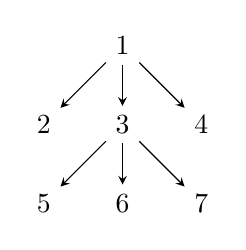
\begin{tikzpicture}[auto,node distance=1cm] 
    \node (1) {1};
    \node [below of=1] (3) {3};
    \node [left of=3] (2) {2};
    \node [right of=3] (4) {4};
    \node [below of=3] (6) {6};
    \node [left of=6] (5) {5};
    \node [right of=6] (7) {7};
    
    \path (1) edge[cfgedge] (2); 
    \path (1) edge[cfgedge] (3);
    \path (1) edge[cfgedge] (4);
    \path (3) edge[cfgedge] (5);
    \path (3) edge[cfgedge] (6);
    \path (3) edge [cfgedge](7);
    \end{tikzpicture}
    \caption{Dominator tree $T_1$}
    \label{fig:tree1}
  \end{figure}
  % 3
  \item (3 points) Consider the dominator tree $T_1$ in
  Figure~\ref{fig:tree1}. Draw \textbf{one} control-flow graph whose
  dominator tree is $T_1$. Recall that a control-flow graph (CFG) has a
  single entry node (a node with no incoming edges), a single exit node (a
  node with no outgoing edges), and all nodes are reachable from the entry
  node. 
  \begin{mdframed}
    \begin{tikzpicture}[
          node distance=1.5cm and 2cm,
          every node/.style={draw, ellipse, minimum width=1.2cm, minimum height=1cm, align=center},
          arrow/.style={draw, -{Latex[length=2mm]}, thick}
        ]
        
        % Nodes
        
        \node (n1) [below=of entry] {1};
        \node (n2) [below left=of n1] {2};
        \node (n4top) [below right=of n1] {4};
        \node (n3) [below=of n1] {3};
        \node (n7) [below left=of n3] {7};
        \node (n6) [below=of n3] {6};
        \node (n5) [below right=of n3] {5};
        
        
        % Arrows
       
        \draw[arrow] (n1) -- (n2);
        \draw[arrow] (n1) -- (n4top);
        \draw[arrow] (n1) -- (n3);
        \draw[arrow] (n2) -- (n3);
        \draw[arrow] (n4top) -- (n3);
        \draw[arrow] (n3) -- (n7);
        \draw[arrow] (n3) -- (n5);
        \draw[arrow] (n3) -- (n6);
        \draw[arrow] (n7) -- (n6);
        \draw[arrow] (n5) -- (n6);
        
    
    \end{tikzpicture}
  \end{mdframed}

  \clearpage
  \item (5 points) State whether the following statement is \textbf{True} or
  \textbf{False}: 

    \emph{Given a flow graph $G$, if there is an control-flow edge from node
    $u$ to node $v$, then the immediate dominator of $v$ dominates $u$.}

  If \textbf{True}, provide a proof.
  If \textbf{False}, provide a counter-example in the form of the flow graph
  $G$ and the nodes $u$~and~$v$.
  \begin{mdframed}
    %\vspace{2em}
    %% \textbf{True} PROVIDE PROOF
    The statement is True, and we will do a proof by contradiction to prove this below.

    Assume that given a flow graph $G$, if there is a control-flow edge from node
    $u$ to node $v$, then the immediate dominator of $v$ does NOT dominate $u$
    
    An immediate dominator of $v$ is defined as a unique strict dominator of $v$ that does not dominate any other strict dominators of $v$. 

    We can assume there exists a control-flow edge from node $u$ to node $v$, where the immediate dominator of $v$ does NOT dominate $u$.

    Lets call the immediate dominator $d$. That means the only way to get to $v$ is through $d$ and there is no other dominator of $v$ in between $d$ and $v$. 

    Since we know $d$ is not dominator of $u$ and there is a control flow edge between $u$ and $v$ this means that there is a path $p$ from entry to $v$ that does not pass through $d$.

    However this leads to a contradiction because we already stated that $d$ is a dominator of $v$.
        
        
    %% \textbf{False} PROVIDE COUNTER-EXAMPLE
  \end{mdframed}

  \clearpage
  \begin{figure}[h]
    \centering
    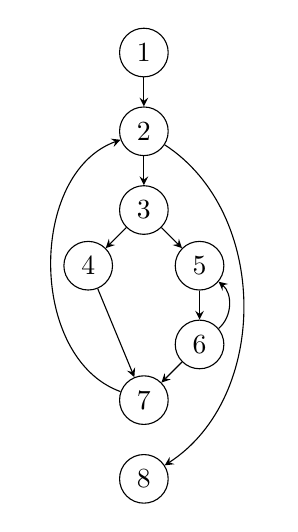
\begin{tikzpicture}[auto,node distance=1cm] 
    \tikzstyle{every node} = [circle, draw]
    \node (1) {1};
    \node [below of=1] (2) {2};
    \node [below of=2] (3) {3};
    \node [below left of=3] (4) {4};
    \node [below right of=3] (5) {5};
    \node [below of=5] (6) {6};
    \node [below left of=6] (7) {7};
    \node [below of=7] (8) {8};
    
    \path (1) edge[cfgedge] (2); 
    \path (2) edge [cfgedge,bend left=57] (8);
    \path (2) edge[cfgedge] (3);
    \path (3) edge[cfgedge] (4);
    \path (3) edge[cfgedge] (5);
    \path (4) edge[cfgedge] (7);
    \path (5) edge [cfgedge](6);
    \path (6) edge[cfgedge,bend right=50] (5);
    \path (6) edge[cfgedge] (7);
    \draw (7) edge [cfgedge, bend left=70] (2);
    \end{tikzpicture}
    \caption{Directed graph $G$}
    \label{fig:graph1}
  \end{figure}
  \item (10 points) The route of the search in a depth-first search of a
  directed graph forms a \emph{depth-first spanning tree (DFST)}. When we
  construct a DFST for a flow graph, the edges of the flow graph fall into
  three categories (i)~\emph{advancing edges}: edges that go from a node $m$
  to a proper descendent of $m$ in the tree, (ii)~\emph{retreating edges}:
  edges that go from a node $m$ to an ancestor of $m$ in the tree (possibly
  to $m$ itself), and (iii)~\emph{cross edges}: edges $m \cfgarrow n$ such
  that $m$ nor $n$ is an ancestor of the other in the DFST.

  The DFST representation of graph $G$ (Figure~\ref{fig:graph1}) is shown in
  Figure~\ref{fig:dfst1}. Advancing edges for indicated using $\cfgarrow$,
  retreating edges using $ \backwardarrow $, and cross edges using
  $\forwardarrow$.

  \begin{figure}[h]
    \centering
    \begin{subfigure}[b]{0.50\linewidth}
      \centering
        
      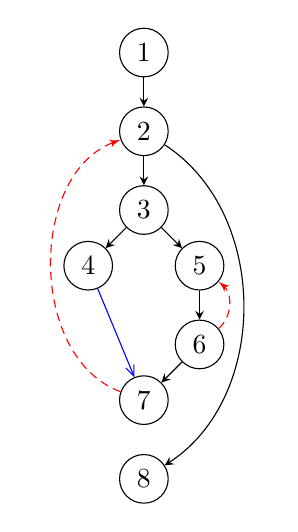
\begin{tikzpicture}[auto,node distance=1cm] 
      \tikzstyle{every node} = [circle, draw]
      \node (1) {1};
      \node [below of=1] (2) {2};
      \node [below of=2] (3) {3};
      \node [below left of=3] (4) {4};
      \node [below right of=3] (5) {5};
      \node [below of=5] (6) {6};
      \node [below left of=6] (7) {7};
      \node [below of=7] (8) {8};
      
      \path (1) edge[cfgedge] (2); 
      \path (2) edge [cfgedge,bend left=57] (8);
      \path (2) edge[cfgedge] (3);
      \path (3) edge[cfgedge] (4);
      \path (3) edge[cfgedge] (5);
      \path (4) edge[forward] (7);
      \path (5) edge [cfgedge](6);
      \path (6) edge[backward,bend right=50] (5);
      \path (6) edge[cfgedge] (7);
      \draw (7) edge [backward, bend left=70] (2);
      \end{tikzpicture}
    \caption{DFST representation of graph $G$ (Figure~\ref{fig:graph1}).}
    \label{fig:dfst1}
    \end{subfigure}
    %
    \begin{subfigure}[b]{0.40\linewidth}
      \centering
  
      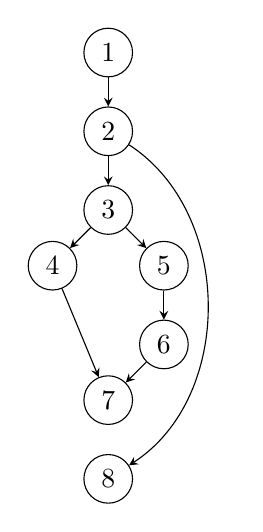
\begin{tikzpicture}[auto,node distance=1cm] 
      \tikzstyle{every node} = [circle, draw]
      \node (1) {1};
      \node [below of=1] (2) {2};
      \node [below of=2] (3) {3};
      \node [below left of=3] (4) {4};
      \node [below right of=3] (5) {5};
      \node [below of=5] (6) {6};
      \node [below left of=6] (7) {7};
      \node [below of=7] (8) {8};
      
      \path (1) edge[cfgedge] (2); 
      \path (2) edge [cfgedge,bend left=57] (8);
      \path (2) edge[cfgedge] (3);
      \path (3) edge[cfgedge] (4);
      \path (3) edge[cfgedge] (5);
      \path (4) edge[cfgedge] (7);
      \path (5) edge [cfgedge](6);
      \path (6) edge[cfgedge] (7);
      \end{tikzpicture}
    \caption{Graph $G_T^-$. }
    \label{fig:graphminus}
    \end{subfigure}
  \end{figure}
  Given a flow graph $G$ and a DFST $T$, let $G_T^-$ denote the flow graph
  produced by removing all retreating edges from G; advancing and cross
  edges are retained. Figure~\ref{fig:graphminus} shows $G_T^-$ for the flow
  graph in Figure~\ref{fig:graph1} given the DFST in Figure~\ref{fig:dfst1}.
  Notice that the dominator tree of $G$ is the same as that for $G_T^-$.

  State whether the following statement is \textbf{True} or \textbf{False}: 

  \emph{Given a flow graph $G$ and a DFST $T$, the dominator tree for $G$ is
  the same as the dominator tree for $G_T^-$.}

  If \textbf{True}, provide a proof.
  If \textbf{False}, provide a counterexample in the form of the flow graph $G$, the DFST $T$, and the dominator trees for $G$  and $G_T^-$.

  \begin{mdframed}

    %% TODO
    %% \textbf{True} PROVIDE PROOF
           \vspace{.5em}

    The above claim is true and we can prove this through a proof by contradiction.
    
           \vspace{.5em}

    Assume for contradiction that Given a flow Graph G and a DFST T, the dominator tree for G \textbf{does} change with the removal of all retreating edges.

    \vspace{0.5em}
    
    By the definition of the dominator relation, we know that $a \dom b$ means that for all paths $p$ from entry to $b$, $p$ must pass through $a$. Now let's remove the retreating edges thus causing our dominator tree to change by our assumption.
     \vspace{0.5em}

    Retreating edges (by definition) go from a node to one of its ancestors in the depth-first spanning tree, and such edges can never be part of a path from the entry node to any other node. Therefore, removing them cannot affect any path that starts at the entry node.
    
   \vspace{.5em}
   
    Since dominator relationships are defined based only on paths from the entry node, the presence or absence of retreating edges cannot affect which nodes dominate others. This means removing the retreating edge from $b$ would not affect the dominator relation of its ancestor to any other node. 

          \vspace{.5em}

    This means that the only dominator relation in the dominator tree that will be affected will between $a$ and $b$. The only ways for the dominator tree to change would be if there was an additional relation caused or there was a dominator relation removed. It is clear that a dominator relation cannot be added since we are \textbf{removing} an edge, thus there cannot be any additional paths resulting from this.

     \vspace{.5em}

    If a dominator relation is removed, that means either the dominator set of $b$ has changed or of $a$ has changed. By definition, $b$ cannot dominate its ancestor, because you have to traverse \textit{through} the ancestor to reach $b$, so an ancestor can never be in the dominator set to begin with. Therefore, the set of nodes that $b$ dominates does not change.
    
   \vspace{.5em}
   
    If we say that $a$ is no longer in the dominator set of $b$ that means that there is some path from entry to $b$ that avoids $a$. This means that $a$ is no longer an ancestor of $b$. This contradicts the assumption, because removing a retreating edge cannot remove any path from the entry to $b$, so $a$ must still dominate $b$. 

       \vspace{.5em}

    Since we reach a contradiction, we have proved that removing retreating edges in a CFG $G$ does not change the dominator tree.
           \vspace{.5em}

    
    %% \textbf{False} PROVIDE COUNTER-EXAMPLE
  \end{mdframed}
\vspace{.5em}

  \item (5 points) State whether the following statement is \textbf{True} or
  \textbf{False}: 

  \emph{Given a flow graph $G$, if node $a$ dominates node $b$, then $b$ post-dominates $a$.}

  If \textbf{True}, provide a proof. If \textbf{False}, provide a
  counter-example in the form of the flow graph $G$ and the nodes
  $a$~and~$b$.
  \begin{mdframed}
    %%\vspace{2em}
    %% TODO
    %% \textbf{True} PROVIDE PROOF
   % This statement is true and a proof will be given below.

    % \vspace{0.5em}
    
    % We can prove this through contradiction. Assume for contradiction that given a flow graph $G$, if node $a$ dominates node $b$, then $b$ does \textbf{not} post-dominates $a$.
    
    % \vspace{0.5em}
    
    % The definition of $a \dom b$ (a dominates b) means every path $p$ from the start node to node $b$ passes through node $a$.
    
    % Similarly the definition of $a$ post dominates $b$ states that every path $p$ from $a$ to exit must pass through $b$.
    
    % \vspace{0.5em}
    
    % Through our assumption, if $b$ does not post dominate $a$ that means there is some path $p$ that exists such that $p$ does not pass through $b$ to get to the exit

    
    \textbf{False} 
    
    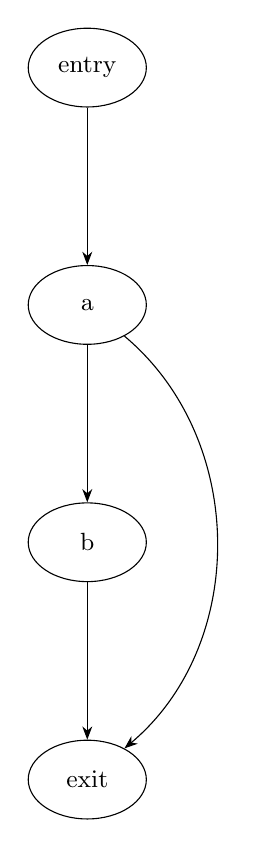
\begin{tikzpicture}[
        node distance=2cm,
        every node/.style={draw, ellipse, minimum width=1.5cm, minimum height=1cm, font=\small},
        ->, >=Stealth
    ]
    
    % Nodes
    \node (entry) {entry};
    \node[below=of entry] (a) {a};
    \node[below=of a] (b) {b};
    \node[below=of b] (exit) {exit};
    
    % Edges
    \draw (entry) -- (a);
    \draw (a) -- (b);
    \draw (a) to[bend left=50] (exit);
    \draw (b) -- (exit);
    
    \end{tikzpicture}
    
  \end{mdframed}
  

  \item  Consider the following algorithm for computing the dominator
  relation for a CFG with nodes $\{1,2,\dots,n\}$:

  {\centering
  \begin{minipage}{.9\linewidth}
    \begin{algorithm}[H]
      \SetAlgoRefName{1}
      \SetKwData{domKw}{DOM}
      \SetKw{returnKw}{return}
      \DontPrintSemicolon
      \KwIn{Directed graph $G$ with nodes $\{1,2,\dots,n\}$, sequence $L$ of graph nodes}

      \KwOut{Dominators $\domKw$ }
   
      \ForEach{$v \in \{1, 2, \dots, n\}$} {
        $\domKw[v] \coloneqq \{1, 2, \dots, n\}$
      }
      \ForEach{$v \in L$} {
        $\domKw[v] \coloneqq \big( \bigcap_{p \in pred(v)} \domKw[p] \big) \cup \{v\}$\label{li:update}
      }
      \returnKw{$\domKw$}
    \caption{ComputeDominator($G$, $L$)}
    \label{alg:dom}
    \end{algorithm}
  \end{minipage}
  \par
  }

  The above algorithm is similar to the iterative dominator algorithm
  discussed in class; in particular, the update to $DOM[v]$ on
  line~\ref{li:update} is the same. However, instead of iterating over all
  the nodes until fixpoint, the above algorithm merely traverses the nodes
  in $L$ once. It should be clear that the correctness and performance of
  the above algorithm depends entirely on the list $L$ passed as input. We
  refer to a sequence $L$ that can be used by Algorithm~\ref{alg:dom} to
  correctly compute dominators for the graph $G$ as a \emph{dominator
  sequence} for $G$.

  \begin{figure}[t]
    \centering
    \begin{subfigure}[b]{0.50\linewidth}
      \centering
      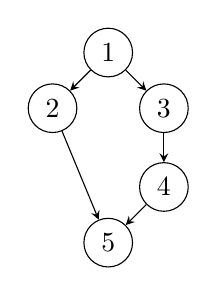
\begin{tikzpicture}[auto,node distance=1cm]
      \tikzstyle{every node} = [circle, draw]
      \node (1) {1};
      \node [below left of=1] (2) {2};
      \node [below right of=1] (3) {3};
      \node [below of=3] (4) {4};
      \node [below left of=4] (5) {5};
      
      \path (1) edge[cfgedge] (2);
      \path (1) edge[cfgedge] (3);
      \path (2) edge[cfgedge] (5);
      \path (3) edge [cfgedge](4);
      \path (4) edge[cfgedge] (5);
      \end{tikzpicture}
    \caption{Graph $G_2$}
    \label{fig:graph2}
    \end{subfigure}
    %
    \begin{subfigure}[b]{0.40\linewidth}
      \centering
      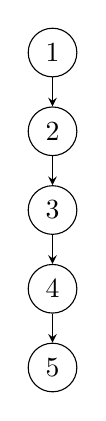
\begin{tikzpicture}[auto,node distance=1cm]
      \tikzstyle{every node} = [circle, draw]
      \node  (3) {1};
      \node [below  of=3] (4) {2};
      \node [below  of=4] (5) {3};
      \node [below of=5] (6) {4};
      \node [below of=6] (7) {5};
      
      \path (3) edge[cfgedge] (4);
      \path (4) edge[cfgedge] (5);
      \path (5) edge [cfgedge](6);
      \path (6) edge[cfgedge] (7);
      \end{tikzpicture}
    \caption{Graph $G_3$}
    \label{fig:graph3}
    \end{subfigure}
  \caption{}
  \end{figure}

  For the graph $G_2$ (Figure~\ref{fig:graph2}), the sequence $[1,2,3,4,5]$
  is a dominator sequence and so is the sequence $[1,3,2,4,5]$.
  The sequence $[1, 2,3,5,4]$ is NOT a dominator sequence, while
  the sequence $[1,2,3,5,4,5]$ is a dominator sequence. 
  
  \begin{enumerate} 
    \item (4 points) List the \emph{shortest} dominator sequence for the
    graph $G$ in Figure~\ref{fig:graph1}.
    \begin{mdframed}
      %% TODO
      $L = [1,2,3,4,5,6,7,8]$
    \end{mdframed}

    \item (4 points) List the \emph{shortest} dominator sequence for the
    graph $G_3$ in Figure~\ref{fig:graph3}.
    \begin{mdframed}
      
      $L = [1,2,3,4]$
    \end{mdframed}

    \item (10 points) State whether the following statement is \textbf{True}
    or \textbf{False}: 

      \emph{The length of the shortest dominator sequence for any flow graph
      $G$ with $N$ nodes is at most $N$.}

    If \textbf{True}, provide a proof. If \textbf{False}, provide a
    counter-example in the form of the flow graph $G$ and the shortest
    dominator sequence $L$.
    \begin{mdframed}
      %%\vspace{15em}
      %% TODO
       \textbf{True}

From our previous proof, we know that a Control Flow Graph (CFG) $G$ and $G-$ share the same dominator relationships, where $G-$ is the CFG $G$ but with all retreating edges removed. Therefore, for the purpose of this proof, we assume that every CFG $G$ has an equivalent CFG $G-$ because any CFG can be translated into $G-$ without affecting the structure of its dominator tree.

   As shown above in the pseudocode for ComputesDominator, the dominator algorithm computes the correct dominator sets in a single pass, provided that every time we examine a node, it's predecessors already have correct dominator information. This is seen in the line 4 where we intersect the dominator sets for all $p$ predecessors. It is clear from this line that if the dominator sets for all the predecessors is correct, then the dominator set for the successor will be correct, since all the predecessors will have the correct information.

    We can exploit this to generate a valid dominator sequence. Since $G-$ is just $G$ but without any of the retreating edges, we can say it is acyclic—i.e., a node \( x \) cannot have a descendant \( y \) that is also a predecessor of \( x \). In other words, there are no cycles.

    Thus, we want to schedule the nodes so that whenever a node is processed, all of its predecessors have already been processed and have valid dominator information. This scheduling can be achieved using a dependency graph:

    \begin{itemize}
      \item For each node \( n \) in $G-$:
      \begin{itemize}
        \item For each predecessor \( p \) of \( n \), add a directed edge from \( n \) to \( p \) in the dependency graph.
      \end{itemize}
    \end{itemize}

    After constructing this dependency graph, we perform a topological sort. The resulting ordering ensures that every node appears after its predecessors, guaranteeing that when we compute the dominators of a node, all necessary data is already available.

    This algorithm is correct because it explicitly encodes the dependency of each node on its predecessors. The topological sort then provides a valid sequence for dominator computation.

    Since the dependency graph contains \( N \) nodes, the topological sort will always yield a sequence of length \( N \). However, in practice, we can sometimes shorten this sequence by omitting nodes whose dominator sets remain at the initialized value (i.e., all nodes in the graph). These nodes don't need to appear in the sequence.

    Therefore, we have shown that the dominator sequence of any CFG with \( N \) nodes is of length at most \( N \).

      
      %% \textbf{False} PROVIDE COUNTER-EXAMPLE
    \end{mdframed}
  \end{enumerate}

  \item State whether the following statements are \textbf{True} or
  \textbf{False}:
  \begin{enumerate}
    \item (3 points) \emph{For all nodes $x, y$ in a CFG, if node $x$ is
    control dependent on node $y$, \\
    then there is a path from $y$ to $x$ in the CFG.}

    If \textbf{True}, provide a proof.
    If \textbf{False}, provide a counter-example in the form of the flow
    graph $G$ and and nodes $x$ and $y$.
    \begin{mdframed}
      
      %% TODO
      \textbf{True}

      \vspace{0.5em}

      We can prove this using a direct proof, shown below.

      \vspace{0.5em}

      From the definition of control dependence, we know that if $x$ is control dependent on $y$, that means that $x$ post dominates a \textbf{successor} of $y$ \textbf{and} $x$ \textbf{does not} strictly post dominate $y$.

      \vspace{0.5em}

      Let's call $s$ the successor of $y$. This means, by definition, that there is a path from $y$ that connects to $s$. We also know that $x$ post dominates $s$. By definition, post domination means that \textbf{all paths $p$} from the current node to the exit \textbf{must} pass through the post dominator. In this case that means \textbf{for all paths $p$} that start from the successor $s$  to exit, $p$ \textbf{must} pass through $x$, by definition.

      \vspace{0.5em}

      We have just established that by the definition of a successor, there is a path from $y$ to successor $s$, and by the definition of a post dominator, all paths from $s$ must pass through $x$. Since this is the case, it follows that there exists some path from $y$ to $x$ in the CFG.

     \vspace{0.5em}

     Therefore, we have proven the claim true and we are done.
      %% \textbf{False} PROVIDE COUNTER-EXAMPLE
    \end{mdframed}
  
    \item (3 points)
    \emph{For all nodes $x, y$ in a CFG, if node $x$ is control dependent on
    node $y$, then node $y$ is NOT control dependent on node $x$.}

    If \textbf{True}, provide a proof.
    If \textbf{False}, provide a counter-example in the form of the flow
    graph $G$ and and nodes $x$ and $y$.
    \begin{mdframed}
      %% TODO
      %% \textbf{True} PROVIDE PROOF
      \textbf{False} The following graph shows $x$ is control dependent on $y$ and $y$ is control dependent on $x$

    \begin{tikzpicture}[
        node distance=2.5cm and 2.5cm,
        every node/.style={draw, ellipse, minimum width=1.5cm, minimum height=1cm},
        ->, >=Stealth
      ]
    
      \node (entry) {entry};
      \node (x) [below=of entry] {x};
      \node (y) [below left=of x] {y};
      \node (z) [below right=of x] {z};
      \node (s) [below=of y] {s};
      \node (exit) [below=of z] {exit};
    
      \draw (entry) -- (x);
      \draw (x) -- (y);
      \draw (x) -- (z);
      \draw (y) -- (s);
      \draw (s) -- (z);
      \draw (z) -- (exit);
      
      % Add separate edges between x and y
      \draw[->, bend left=30] (y) to (x);  % Curved edge from x to y
    
    \end{tikzpicture}


    \end{mdframed}
  
    \item (3 points) \emph{For all nodes $x, y, z$ in a CFG, if node $x$ is
    control dependent on node~$y$, and node $y$ is control dependent on
    node~$z$, then node $x$ is control dependent on node $z$.}

    If \textbf{True}, provide a proof. If \textbf{False}, provide a
    counter-example in the form of the flow graph $G$ and and nodes $x$,
    $y$, and $z$.
    \begin{mdframed}
      %% TODO
      %% \textbf{True} PROVIDE PROOF
      \textbf{False}, in the graph below $x$ is control dependent on $y$ and $y$ is control dependent on $z$, but $x$ is not control dependent on $z$ because it does not post dominate a successor of $z$. So it does not fulfill the conditions of being control dependent.

    \begin{tikzpicture}[
        ->, 
        >=Stealth, 
        node distance=1.8cm and 2.5cm, 
        every node/.style={draw, ellipse, minimum width=1.2cm, minimum height=1cm, font=\bfseries}
        ]
    
        % Nodes
        \node (entry) {entry};
        \node (1) [right=of entry] {z};
        \node (2) [below left=of 1] {y};
        \node (3) [below right=of 1] {a};
        \node (4) [below left=of 2] {x};
        \node (5) [below right=of 2] {b};
        \node (exit) [below right=of 4] {exit};
    
        % Edges
        \draw (entry) -- (1);
        \draw (1) -- (2);
        \draw (1) -- (3);
        \draw (2) -- (4);
        \draw (2) -- (5);
        \draw (3) -- (5);
        \draw (4) -- (exit);
        \draw (5) -- (exit);
    
    \end{tikzpicture}
            


    \end{mdframed}
  \end{enumerate}
  
\end{enumerate}

\end{document}
